% Define the document style. The thesis stylesheet inherits from 'report'. 
% I had once made a version inheriting from book. However the two versions are almost 
% compatible. The main difference is that the other version supported 'parts'.
% (extended from book) and this does not.
% IST requires the thesis to be written in Arial or similar. Two arguments allow you 
% to define the thesis font: 'Helvetica' and 'AvantGarde', which transforms normal font
% into Helvetica or AvantGarde, respectively... dahhhh!
\documentclass[defaultstyle,10pt,a4paper,master,Helvetica]{thesis}
%\documentclass[defaultstyle,12pt,phd]{thesis}

% Defines an additional alphabet... not required in most cases
% ------------------------------------------------------------
% \DeclareMathAlphabet{\mathpzc}{OT1}{pzc}{m}{it}

% PACKAGE fontenc:
% -----------------
% chooses T1-fonts and allows correct automatic hyphenation.
\usepackage[T1]{fontenc}
\usepackage[latin1]{inputenc}

% PACKAGE babel:
% ---------------
% The 'babel' package may correct some hyphenisation issues of latex. 
% However in most situations it is not required.
\usepackage[portuges]{babel}

% PACKAGE latexsym:
% -----------------
% Defines additional latex symbols. May be required for thesis with many math symbols.
%\usepackage{latexsym}

% PACKAGE amsmath, amsthm, amssymb, amsfonts:
% -------------------------------------------
% This package is typically required. Among many other things it adds the possibility
% to put symbols in bold by using \boldsymbol (not \mathbf); defines additional 
% fonts and symbols; adds the \eqref command for citing equations. I prefer the style
% "(x.xx)" for referering to an equation than to use "equation x.xx".
\usepackage{amsmath, amsthm, amssymb, amsfonts}

% PACKAGE multirow, colortbl, longtable:
% ---------------------------------------
% These packages are most usefull for advanced tables. The first allows to join rows 
% throuhg the command \multirow which works similarly with the command \multicolumn
% The second package allows to color the table (both foreground and background)
% The third package is only required when tables extend beyond the length of one page;
% which typically does not happen and should be avoided
\usepackage{multirow}
\usepackage{colortbl}
% \usepackage{longtable}

% PACKAGE graphics, epsfig, subfigure, caption:
% ---------------------------------------------
% Packages for figures... well you will certainly need these packages, with the exception
% of the 'caption' package. This only allows to define extra caption options.
% Notice that subfigure allows to place figures within figures with its own caption. It
% should be avoided to create an eps file with subfigures. That will mean that you won't be 
% able to reference those subfigures. Instead create an EPS file (the only graphics format supported
% by latex) for each of the subfigures and then use the command \subfigure (see below).
\usepackage{graphicx}
\usepackage{epsfig}
\usepackage[hang,small,bf]{subfigure}
% \usepackage[hang,small,bf]{caption}

% PACKAGE algorithmic, algorithm
% ------------------------------
% These packages are required if you need to describe an algorithm.
% \usepackage{algorithmic}
% \usepackage[chapter]{algorithm}

% PACKAGE natbib/cite
% -------------------
% The two packages are not compatible, and you should use one of the two. Notice however that the
% IEEE BiBTeX stylesheet is imcompatible with the natbib package. If using the IEEE format, use the 
% cite package instead
\usepackage[square,numbers,sort&compress]{natbib}
%\usepackage{cite}

% PACKAGE acronyum
% -----------------
% This package is most usefull for acronyms. The package garantees that all acronyms definitions are 
% given at the first usage. IMPORTANT: do not use acronyms in titles/captions; otherwise the definition 
% will appear on the table of contents.
\usepackage[printonlyused,withpage]{acronym}

% PACKAGE extra_functions
% -----------------
% My Personal package: defines the following commands:
% \fancychapter{chaptername) -> Prints a fancier chapter (you can also use the fancychapter package for this)
% \hline{width} -> use for a replacement of the \hline command
% \Mark1, \Mark2, \Mark3, ...
\usepackage{extra_functions}

% PACKAGE tocloft
% -----------------
% The tocloft package provides means of controlling the typographic design of the Table of Contents,
% List of Figures and List of Tables. New kinds of `List of . . . ' can be defined.
% The package has been tested with the tocbibind, minitoc, ccaption, subfigure, float, fncychap, and hyperref packages.
\usepackage[subfigure]{tocloft}

% PACKAGE babelbib
% -----------------
\usepackage[fixlanguage]{babelbib}
\selectbiblanguage{portuges}

% PACKAGE todonotes
% -----------------
% \usepackage{todonotes}

% PACKAGE IEEEtrantools
% -----------------
% Allows customization of the IEEEtran bibliography style
% \usepackage[retainorgcmds]{IEEEtrantools}

% PACKAGE fixltx2e
% -----------------
% Allows the \textsubscript{} command, among other fixes
\usepackage{fixltx2e}

% PACKAGE longtable
% -----------------
% Use this instead of tabular when you need footnotes inside a table
\usepackage{longtable}

% PACKAGE hyperref
% -----------------
% Set links for references and citations in document
% Some MiKTeX distributions have faulty PDF creators in which case this package will not work correctly
% Long live Linux :D
\usepackage{hyperref}
\hypersetup{ a4paper=true,
             colorlinks=false,
             citecolor=red,
             breaklinks=true,
%            bookmarks=true,		% commented because it generated a warning
             bookmarksnumbered=true,
             bookmarksopen=true,
             pdftitle={T�tulo do PDF},
             pdfauthor={Autor},
             pdfsubject={Tese de Mestrado},
             pdfcreator={LaTeX},
             pdfkeywords={}
}

\def\chapterautorefname{Cap�tulo}
\def\sectionautorefname{Sec��o}
\def\subsectionautorefname{Subsec��o}
\def\figureautorefname{Figura}
\def\tableautorefname{Tabela}

% PACKAGE hypcap
% -----------------
% In case you use the package hyperref to create a PDF, the links to tables or figures
% will point to the caption of the table or figure, which is always below the table or figure itself.
% Therefore the table or figure will not be visible, it is above the pointer and one has
% to scroll up in order to see it.
% If you want the link point to the top of the image you can use this package
\usepackage[all]{hypcap}

% PACKAGE breakurl
% -----------------
% Provides breakable URLs
% This package is designed to be loaded after hyperref to provide a breakable
% hyperlinked \url command under DVI output
%
% Note: apparently not needed when using pdfTeX
% \usepackage{breakurl}

% Set paragraph counter to alphanumeric mode
\renewcommand{\theparagraph}{\Alph{paragraph}~--}

% Page formatting... It was correct for my master thesis... not sure it is still correct
\hoffset 0in
\voffset 0in
\oddsidemargin 0.71cm
\evensidemargin 0.04cm
\marginparsep 0in
\topmargin -0.25cm
\textwidth 15cm
\textheight 23.5cm

\usepackage{fancyhdr}
\pagestyle{fancy}
\renewcommand{\chaptermark}[1]{\markboth{\thechapter.\ #1}{}}
\renewcommand{\sectionmark}[1]{\markright{\thesection\ #1}}
\fancyhf{} \fancyhead[LE]{\bfseries\nouppercase{\leftmark}}
\fancyhead[RO]{\bfseries\nouppercase{\rightmark}}
\fancyfoot[LE,RO]{\bfseries\thepage}
\renewcommand{\headrulewidth}{0.5pt}
\renewcommand{\footrulewidth}{0.5pt}
\addtolength{\headheight}{2pt} % make space for the rule
\fancypagestyle{plain}{%
   \fancyhead{} % get rid of headers
   \renewcommand{\headrulewidth}{0pt} % and the line
   \renewcommand{\footrulewidth}{0pt}
}
\fancypagestyle{blank}{%
   \fancyhf{} % get rid of headers and footers
   \renewcommand{\headrulewidth}{0pt} % and the line
   \renewcommand{\footrulewidth}{0pt}
}
\fancypagestyle{abstract}{%
   \fancyhead{}
   \renewcommand{\headrulewidth}{0pt}
   \renewcommand{\footrulewidth}{0.5pt}
}
\fancypagestyle{document}{%
	\fancyhf{} \fancyhead[LE]{\bfseries\nouppercase{\leftmark}}
	\fancyhead[RO]{\bfseries\nouppercase{\rightmark}}
	\fancyfoot[LE,RO]{\bfseries\thepage}
	\renewcommand{\headrulewidth}{0.5pt}
	\renewcommand{\footrulewidth}{0.5pt}
	\addtolength{\headheight}{2pt} % make space for the rule
}
\setcounter{secnumdepth} {5}
\setcounter{tocdepth} {5}
\renewcommand{\thesubsubsection}{\thesubsection.\Alph{subsubsection}}

\renewcommand{\subfigtopskip}{0.3 cm}
\renewcommand{\subfigbottomskip}{0.2 cm}
\renewcommand{\subfigcapskip}{0.3 cm}
\renewcommand{\subfigcapmargin}{0.2 cm}


% Custom commands for automatic text
% (remember to add {} after each one, or adjacent spaces will be suppressed)
\newcommand{\isocless}{\mbox{ISO/IEC 14443}}
\newcommand{\extlog}{\textit{Extended Logging}}
\newcommand{\emv}{\nameref{sec:ea:emv}}

\newcommand{\acroemph}[1]{\textit{#1}}

\begin{document}

% This solves a pdfTeX warning about page counters related to hyperref
% See: http://en.wikibooks.org/wiki/LaTeX/Packages/Hyperref#Problems_with_Links
\pagenumbering{alph}

% Add PDF bookmark 
\pdfbookmark[0]{Capa}{Titlepage}

%%%%%%%%%%%%%%%%%%%%%%%%%%%%%%%%%%%%%%%%%%%%%%%%%%%%%%%%%%%%%%%%%%%%%%%%%%%%%%%%%%%%%%%%%%%%%%%%
% DEFINE THE TITLEPAGE
% remember that IST requires for the titlepage to be written in portuguese
%%%%%%%%%%%%%%%%%%%%%%%%%%%%%%%%%%%%%%%%%%%%%%%%%%%%%%%%%%%%%%%%%%%%%%%%%%%%%%%%%%%%%%%%%%%%%%%%
% REQUIRED:
% The university logo image: first and second arguments are the (top,left) position of the logo. 
% IST rules force it to be 2cm
\univlogo{3cm}{2cm}{pdf/0_logo_ist_web.pdf}
% OPTIONAL:
% The thesis logo image: first and second arguments are the position of the logo. 
%\thesislogo{2.5cm}{6cm}{img/0_cover_image.png}

% Thesis title
\title{Monitoriza��o Wireless de Pessoas em Ambiente Dom�stico}

% Author and highest current degree (not the one you are applying to)
\author{M�rcio Lu�s Mendon�a de Vasconcelos de N�brega}
\degree{Engenharia Electrot�cnica e de Computadores}
% This is not on the new IST MSc stylesheet... however for PhD dissertations it will most likely be required
% \otherdegree{Mestre}

% The supervisor. Use the second command if required.
% Always remember that 'Professor' should only be used for a supervisor with a Cathedra
\supervisor{Prof. Doutor Renato Jorge Caleira Nunes}
\othersupervisor{Prof. Doutor Ant�nio Manuel Raminhos Cordeiro Grilo}

% Date of the dissertation
\date{Outubro 2012}

% Is this the final version? Place false when delivering the first part.
% The juri members will not be printed in that case. Place true after the juri has accepted the thesis
\finalthesis{true}

% The members of the Juri
% Always remember that 'Professor' should only be used for a juri member with a Cathedra
\presidentofjury{Prof. Doutor Nuno Cavaco Gomes Horta}
\vogalone{Prof. Doutor Carlos Nuno da Cruz Ribeiro}
%\vogaltwo{\_\_\_\_\_\_\_\_\_\_\_\_\_\_\_\_\_\_\_\_\_\_\_\_\_\_\_\_\_\_\_\_\_\_\_\_\_\_\_}
% \vogalthree{Doutor whatever full name 4}
% \vogalfour{Doutor whatever full name 5}
%%%%%%%%%%%%%%%%%%%%%%%%%%%%%%%%%%%%%%%%%%%%%%%%%%%%%%%%%%%%%%%%%%%%%%%%%%%%%%%%%%%%%%%%%%%%%%%%

% print titlepage
\maketitle
\clearpage

% Since I am using double sided pages, the second page should be white.
% Remember that when delivering the dissertation, IST requires for the cover to appear twice.
\thispagestyle{empty}
\cleardoublepage

\setcounter{page}{1} \pagenumbering{roman}

\baselineskip 18pt % line spacing: -12pt for single spacing
                   %               -18pt for 1 1/2 spacing
                   %               -24pt for double spacing

\vspace*{.2\textheight}
\begin{quote}
	\begin{center}
%		\textit{``Some funny/whatever quote, if you want to include one. If not, simply comment this part''} --- Author Name\cite[cap. 5, p. 42]{citacao_anw}
		
		\vspace*{.05\textheight}
		
		\textit{``Uma cita��o engra�ada ou algo do g�nero, se queres incluir uma. Caso n�o, comenta esta parte''}
	\end{center}

\end{quote}

\clearpage

\thispagestyle{empty}
\cleardoublepage

\thispagestyle{plain}
\pdfbookmark{Agradecimentos}{Acknowledgments}
\begin{acknowledgments}
Obrigado ao Pedro Tom�s, o autor original do template para \LaTeX\ (vers�o inglesa).
\end{acknowledgments}

\begin{resumo}
O aumento constante da popula��o idosa mundial tem criado uma enorme quantidade de desafios ao desenvolvimento nacional, � sustentabilidade das fam�lias e � capacidade dos sistemas de sa�de de darem suporte � popula��o idosa. � medida que a tecnologia dos sensores wireless evolui, dispositivos de baixo consumo, reduzida largura de banda e capacidade de armazenamento m�dio, surgem no mercado, com custos de aquisi��o bastante reduzidos. A monitoriza��o de ambientes dom�sticos baseada em sensores wireless, fornece um meio seguro e contido para pessoas idosas, permitindo que estas possam viver nas suas casas o m�ximo tempo poss�vel. Este trabalho introduz o \acf{EMoS}, um sistema desenvolvido no \acf{MiXiM},  onde foi implementado um protocolo de encaminhamento \acf{AODV} e um sistema de localiza��o baseado no HORUS, com a finalidade de monitorizar, num ambiente dom�stico, pessoas idosas ou com necessidades especiais. Os resultados obtidos desta investiga��o demonstram a viabilidade de construir um sistema de monitoriza��o para idosos usando um ambiente simulado onde aspectos de hardware comercialmente dispon�vel foram tamb�m discutidos.
\end{resumo}

\begin{palavraschave}
Redes de Sensores, Pessoas Idosas, Protocolos de Encaminhamento, Localiza��o, MiXiM
\end{palavraschave}

\clearpage
\thispagestyle{empty}
\cleardoublepage

\begin{abstract}
The consistent increase in the world's elder population has been putting a lot of challenges regarding national development, sustainability of families and the ability of health care systems to provide for ageing populations. As wireless sensing technology continues to evolve, devices integrating low-power, low-bandwidth radios and a modest amount of storage, emerge due to considerable reduced costs. Wireless sensors based home monitoring systems provide a safe, sound and secure environment for elder people, enabling them to live in their own home as long as possible. This work introduces the \acf{EMoS}, a \acs{MiXiM} based framework, in which an \acf{AODV} protocol has been implemented together with a modified HORUS system, for tracking and monitoring, in a home environment, elder people or people with special needs. The results obtained from this research demonstrate the feasibility to build a monitoring system for elder care using a simulated environment in which several aspects of the hardware commercially available have been also discussed. 
\end{abstract}


\begin{keywords}
Sensor Networks, Elder Care, Routing Protocols, Indoor Location, MiXiM
\end{keywords}

\clearpage
\thispagestyle{empty}
\cleardoublepage

% This is required for the fancy chapters
\dominitoc
\dominilof
% \dominilot %(I'm not using the List of tables)

%%%%%%%%%%%%%%%%%%%%%%%%%%%%%%%%%%%%%%%%%%%%%%%%%%%%%%%%%%%%%%%%%%%%%%
% List of contents
%\renewcommand{\baselinestretch}{1}
\pdfbookmark[0]{�ndice}{index}
\pdfbookmark[1]{Conte�do}{toc}
\tableofcontents
% \contentsline{chapter}{References}{\pageref{bib}}
\cleardoublepage
%\renewcommand{\baselinestretch}{1.5}

%%%%%%%%%%%%%%%%%%%%%%%%%%%%%%%%%%%%%%%%%%%%%%%%%%%%%%%%%%%%%%%%%%%%%%
% List of figures
\pdfbookmark[1]{Lista de Figuras}{lof}
\listoffigures
\cleardoublepage

%%%%%%%%%%%%%%%%%%%%%%%%%%%%%%%%%%%%%%%%%%%%%%%%%%%%%%%%%%%%%%%%%%%%%%
% List of tables
\pdfbookmark[1]{Lista de Tabelas}{lot}
\listoftables
\cleardoublepage

% %%%%%%%%%%%%%%%%%%%%%%%%%%%%%%%%%%%%%%%%%%%%%%%%%%%%%%%%%%%%%%%%%%%%%%
% % List of algorithms
% Requires packages algorithmic, algorithm
% \pdfbookmark[1]{List of Algorithms}{loa}
% \listofalgorithms
% \cleardoublepage

% %%%%%%%%%%%%%%%%%%%%%%%%%%%%%%%%%%%%%%%%%%%%%%%%%%%%%%%%%%%%%%%%%%%%%%
% % List of acronyms
\pdfbookmark[1]{Lista de Acr�nimos}{loac}

\newcommand{\listacronymsname}{Lista de Acr�nimos}
\newlistof{acronyms}{acr}{\listacronymsname}

\listofacronyms

\begin{acronym}[CDA]
	\acro{BSN}{\acroemph{Body Sensor Network}}
	\acro{BAN}{\acroemph{Body Area Network}}
	\acro{WBAN}{\acroemph{Wireless Body Area Network}}
	\acro{MAC}{\acroemph{Medium Access Control}}
	\acro{GTS}{\acroemph{Guaranteed Time Slots}}
	\acro{WLAN}{\acroemph{Wireless Local Area Network}}
	\acro{WSN}{\acroemph{Wireless Sensor Network}}
	\acro{IR}{\acroemph{Infrared}}
	\acro{CAN}{\acroemph{Car Area Network}}
	\acro{LAN}{\acroemph{Local Area Network}}
	\acro{RFID}{\acroemph{Radio-frequency Identification}}
	\acro{CM}{\acroemph{Case Manager}\acroextra{, profissionais de sa�de do ramo da geriatria.}}
	\acro{ADL}{\acroemph{Activity of Daily Living}}
	\acroplural{ADL}[ADLs]{\acroemph{Activities of Daily Living}}
	\acro{PDA}{\acroemph{Personal Digital Assistant}}
	\acro{BS}{\acroemph{Base Station}}
	\acro{QoS}{\acroemph{Quality of Service}}
	\acro{SPIN}{\acroemph{Sensor Protocolos for Information via Negotiation}}
	\acro{DD}{\acroemph{Direct Diffusion}}
	\acro{AODV}{\acroemph{Ad hoc On-demand Vector Routing}}
	\acro{DSR}{\acroemph{Dynamic Source Routing}}
	\acro{LEACH}{\acroemph{Low-Enegery Adaptive Clustering Hierarchy}}
	\acro{PEGASIS}{\acroemph{Power-Efficient Gathering in Sensor Information Systems}}
	\acro{GEAR}{\acroemph{Geographical and Energy Aware Routing}}
	\acro{TOA}{\acroemph{Time of Arrival}}
	\acro{TDOA}{\acroemph{Time Difference of Arrival}}
	\acro{RSS}{\acroemph{Received Signal Strength}}
	\acro{POA}{\acroemph{Phase of Arrival}}
	\acro{AOA}{\acroemph{Angle of Arrival}}
	\acro{RM}{\acroemph{Radio Map}}
	\acro{RF}{\acroemph{Radio Frequency}\acroextra{, r�dio-frequ�ncia.}}
	\acro{AP}{\acroemph{Access-Point}}
\end{acronym}


\cleardoublepage

% Pages number is starting now with arabic style... until now it was on roman mode
\setcounter{page}{1} \pagenumbering{arabic}
\baselineskip 18pt

% %%%%%%%%%%%%%%%%%%%%%%%%%%%%%%%%%%%%%%%%%%%%%%%%%%%%%%%%%%%%%%%%%%%%%%
% The Introduction:
% %%%%%%%%%%%%%%%%%%%%%%%%%%%%%%%%%%%%%%%%%%%%%%%%%%%%%%%%%%%%%%%%%%%%%%

\fancychapter{Introdu��o}
\label{cap�tulo:introdu��o}
Resumo do cap�tulo.

\section{Motiva��o}
\label{sec��o:introdu��o:motiva��o}
O aumento da esperan�a de vida provoca actualmente um envelhecimento generalizado da popula��o mundial o que coloca diversos desafios ao desenvolvimento nacional, � sustentabilidade das fam�lias e � capacidade dos sistemas de sa�de. Durante anos recentes o n�mero de pessoas no mundo acima dos 60 anos aumentou de 200 milh�es em 1950 para 670 milh�es, sector et�rio que representa j� 20\% da popula��o total nos pa�ses desenvolvidos. \citep{1}. Com a deslocaliza��o das popula��es para os grandes centros, a baixa natalidade, a neglig�ncia familiar, aumenta cada vez mais o n�mero de idosos que vivem sozinhos em suas casas. Esta situa��o cria ansiedade em todos os envolvidos, resultando muitas vezes em internamentos precoces em lares, com um custo elevado e vagas limitadas.

\begin{figure}[!htb]
  \centering
  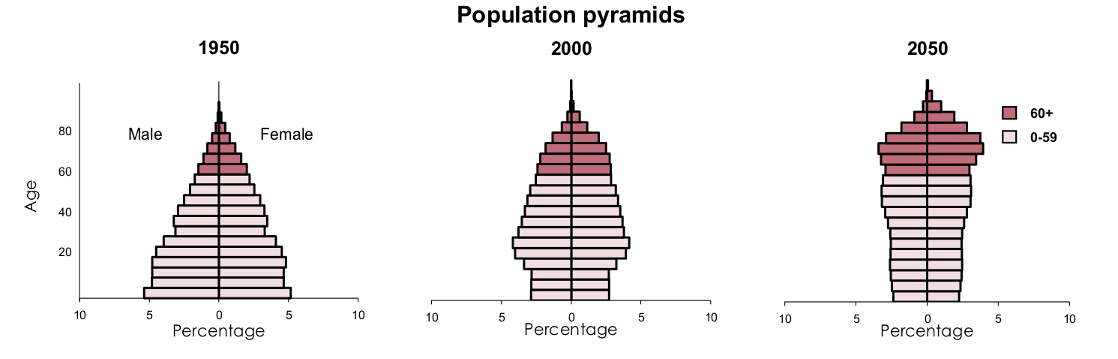
\includegraphics[width=1\textwidth]{img/01_demografia_pt.png}
  \caption{An�lise e previs�o da popula��o em Portugal entre 1950-2050. \cite{1}}
  \label{fig:cap1:demogPT}
\end{figure}

Pessoas com defici�ncias f�sicas ou mentais apresentam tamb�m uma id�ntica necessidade de acompanhamento. Por exemplo, pessoas com defici�ncia mental m�dia, normalmente t�m capacidades sociais e funcionais para serem minimamente independentes, ainda que necessitem de alguma supervis�o e assist�ncia. Normalmente t�m problemas t�o b�sicos como, por exemplo, decidir quando se levantar ou deitar na cama, ou tomar medicamentos � hora certa.

A monitoriza��o de ambos os casos descritos permitiria libertar m�o-de-obra especializada para situa��es de maior depend�ncia, reduzindo custos e aumentando a efici�ncia, notificando m�dicos ou hospitais da mudan�a de sinais vitais que precedam situa��es de risco ou interagindo com ambientes inteligentes.

A evolu��o tecnol�gica dos sensores wireless tem vindo a introduzir no mercado sensores, r�dios e processadores de baixa pot�ncia e baixo custo. Estes dispositivos, com o seu reduzido tamanho, t�m um enorme potencial para o desenvolvimento de aplica��es centradas no utilizador. Com um vasto tipo de sensores, as aplica��es ub�quas\footnote{Aplica��o que tem como objectivo tornar a interac��o entre pessoa e m�quina invis�vel, integrando a inform�tica com ac��es e comportamentos naturais das pessoas.}   podem por isso surgir como alternativa de baixo custo e enorme valor acrescentado para monitoriza��o de pessoas num ambiente dom�stico, criando uma simbiose entre pessoa e m�quina que permita usufruir do direito de viver de forma independente, com privacidade, dignidade e total controlo da pr�pria vida.


\section{Objectivos}
\label{sec��o:introdu��o:objectivos}
Nesta disserta��o � proposto o desenvolvimento de uma solu��o onde uma ou mais pessoas, portadoras de um n� wireless, se movimentam num ambiente onde existem outros n�s wireless. Dever� ser poss�vel localizar cada pessoa e estabelecer uma comunica��o bidireccional entre esta e um servidor central. 

Assim definem-se os seguintes objectivos:
\begin{itemize}
	\item Identificar necessidades num ambiente dom�stico e propor para estas solu��es de hardware existentes no mercado;
	\item Definir a arquitectura do sistema e os papeis de cada interveniente;
	\item Identificar uma plataforma de simula��o existente que permita, de uma forma realista, simular o comportamento do sistema;
	\item Implementar a simula��o de um algoritmo de encaminhamento;
	\item Implementar a simula��o de um algoritmo de localiza��o;
	\item Analisar a simula��o com m�tricas que permitam conhecer o erro de localiza��o, bem como os limites e valores �ptimos do sistema;
\end{itemize}


\section{Principais Contribui��es}
\label{sec��o:introdu��o:contribui��es}
(a escrever no fim)

\section{Organiza��o da Disserta��o}
\label{sec��o:introdu��o:organiza��o}
(a escrever no fim)
%Esta disserta��o encontra-se organizada nos seguintes seis cap�tulos:
%\begin{enumerate}
%	\item \nameref{cap�tulo:introdu��o}
%	\item \nameref{chap:ea}
%	\item \nameref{chap:conclusoes}
%\end{enumerate}
%
%O \autoref{cap�tulo:introdu��o} inclui a introdu��o ao projecto, assim como os seus objectivos, contribui��es do trabalho desenvolvido e a presente explica��o da organiza��o da disserta��o.
%
%O \autoref{chap:ea} ...
%
%Finalmente, no \autoref{chap:conclusoes} s�o tiradas as conclus�es do trabalho efectuado, fazendo-se tamb�m refer�ncias ao trabalho futuro que pode ser feito sobre o apresentado nesta disserta��o.

\cleardoublepage


% %%%%%%%%%%%%%%%%%%%%%%%%%%%%%%%%%%%%%%%%%%%%%%%%%%%%%%%%%%%%%%%%%%%%%%
% Literature Review
% %%%%%%%%%%%%%%%%%%%%%%%%%%%%%%%%%%%%%%%%%%%%%%%%%%%%%%%%%%%%%%%%%%%%%%

\fancychapter{Trabalho Relacionado}
\label{chap:2}
Pequena introdu��o.

\section{Estado da Arte}
\label{chap:2:sec:1}
A gera��o actual de casas inteligentes tem tido uma maior evolu��o na intelig�ncia artificial em sistema centralizado, em detrimento dos sistemas de monitoriza��o e controlo. A casa inteligente actual consiste em v�rios electrodom�sticos e outros dispositivos, com sensores, actuadores e/ou monitores biom�dicos, usados pelos residentes numa base di�ria. Em alguns casos a casa � inteiramente monitorizada recorrendo a tecnologias �udio e v�deo. Estes sistemas apresentam uma excelente forma de monitoriza��o mas t�m algumas desvantagens:

\begin{itemize}
\item Custos elevados devido ao uso de sensores sofisticados e equipamentos �udio-visuais;
\item Custos elevados de instala��o devido � instala��o individualizada;
\item Elevada largura de banda necess�ria;
\item Demasiada intrus�o no quotidiano da pessoa criando um sentimento de falta de privacidade ou desconforto.
\end{itemize}

\subsection{Monitoriza��o com V�deo e �udio}
\label{chap:2:sec:1.1}
Em \cite{2} atrav�s de um sensor wireless equipado com um aceler�metro e transportado pela pessoa, s�o detectadas poss�veis quedas. Por forma a minimizar o n�mero de falsos alarmes, s�o usadas c�maras que cobrem o espa�o, que analisam a posi��o da pessoa e s�o activadas de acordo com uma localiza��o obtida atrav�s de triangula��o baseada nas posi��es conhecidas dos n�s fixos e a pot�ncia recebida pelo n� m�vel. � tamb�m apresentada a possibilidade de efectuar transmiss�o de voz utilizando o r�dio IEEE 802.15.4, uma vez que j� existem r�dios com largura de banda necess�ria para efectuar transmiss�o de voz.

\begin{figure}[!htb]
  \centering
  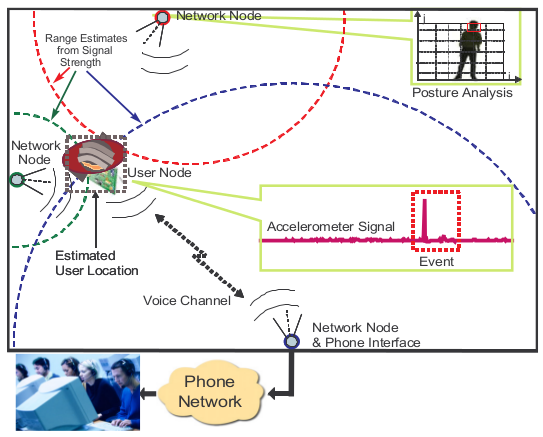
\includegraphics[width=0.50\textwidth]{img/02_video_monit_01.png}
  \caption{Arquitectura do sistema proposto em \cite{2}.}
  \label{fig:1:video_monit_01}
\end{figure}

Em \cite{3} e \cite{4} � feita a combina��o da informa��o fornecida por redes de sensores e sistemas de v�deo-vigil�ncia. Atrav�s de uma infer�ncia l�gica que considera sequ�ncias de eventos s�o tomadas decis�es tal como � poss�vel observar em \ref{fig:2:video_monit_02}. O ocupante da casa usa um sensor n�o intrusivo para determina��o da posi��o e comunica��o por voz, mas n�o � necess�ria qualquer interac��o com a tecnologia. � semelhan�a do trabalho anterior a privacidade � um tema fulcral e todo o tratamento de imagem � feito localmente usando \textit{Smart Cameras} \footnote{c�maras que para al�m de captar imagem tamb�m podem tratar a imagem e obter resultados a partir desta}.

\begin{figure}[!htb]
  \centering
  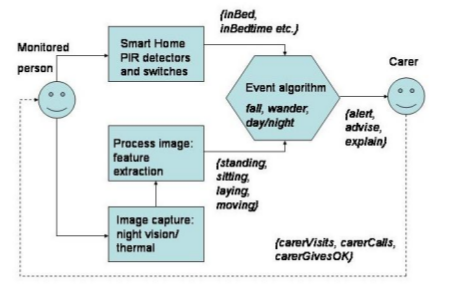
\includegraphics[width=0.75\textwidth]{img/02_video_monit_02.png}
  \caption{Arquitectura de fus�o de decis�o referida em \cite{3}.}
  \label{fig:2:video_monit_02}
\end{figure}

No trabalho \cite{5} � feita a aplica��o de um sistema de monitoriza��o num lar de idosos atrav�s de v�deo e �udio sem recurso a sensores port�teis. O trabalho referencia a insufici�ncia de profissionais em contraste com o r�pido crescimento da popula��o idosa e o pouco tempo que estes t�m dispon�vel para cada idoso. Emerge assim a necessidade de obter um conjunto de dados de forma aut�noma e usado para detectar situa��es de perigo de atempadamente, como por exemplo a instabilidade do andar ou registos comportamentais que favorecem a prescri��o de medicamentos psicotr�picos. Os grandes desafios indicados s�o a localiza��o por v�deo, a correcta identifica��o e marca��o das pessoas no campo de vis�o e a an�lise das suas actividades individuais.

Com fundamento no conceito \textit{aging in place}, onde idosos vivem de forma independente e segura nas suas pr�prias casas, o trabalho \cite{6} apresenta, a monitoriza��o de quedas mas tamb�m funcionalidades utilit�rias como a detec��o de objectos, calend�rio, v�deo-confer�ncia e livro de endere�os. Recorrendo a c�maras e a t�cnicas de \textit{machine learning} o sistema n�o necessita que o utilizador use um sensor. O sistema tem uma abordagem centralizada devido � forte exig�ncia de processamento em tempo real e mem�ria necess�rias. A detec��o de objectos � feita verificando mudan�as na imagem ou procurando objectos de acordo com as suas caracter�sticas. 

\begin{figure}[!htb]
  \centering
  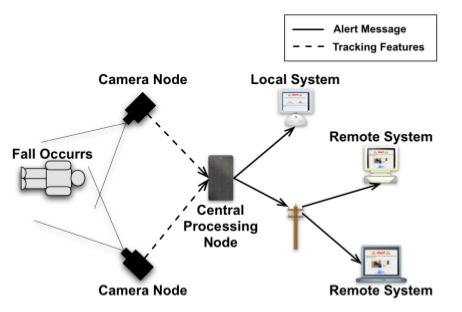
\includegraphics[width=0.7\textwidth]{img/02_video_monit_03.png}
  \caption{Processo de detec��o de quedas e alertas descrito no trabalho \cite{6}.}
  \label{fig:3:video_monit_03}
\end{figure}

Em \cite{7} � utilizado o sinal �udio em conjunto com o v�deo para inferir acerca de uma poss�vel queda. O sinal �udio torna-se essencial para distinguir entre uma pessoa que se sentou ou que caiu. Consideram-se processos de textit{Markov}\footnote{Processo sem mem�ria onde podem ser feitas previs�es do futuro com base somente no 
estado presente, sendo o futuro e passado do processo considerados independentes} que permitem perceber se o comportamento do indiv�duo est� de acordo com o previsto ou n�o e assim tomar as medidas necess�rias.

Embora cada aplica��o tenha as suas mais-valias e a precis�o dos sistemas onde o sinal v�deo � utilizado seja bastante elevada, existe a quest�o da privacidade que resulta numa baixa aceita��o deste tipo de sistemas por parte de pessoas idosas.

A grande preocupa��o nos trabalhos identificados permanece na detec��o de quedas e na fiabilidade dessa detec��o.

\subsection{\textit{Wearable Sensors}}
\label{chap:2:sec:1.2}
Com a evolu��o dos sensores wireless aparecem cada vez mais solu��es que permitem fazer uma monitoriza��o cont�nua do estado de sa�de de uma pessoa, independentemente da sua localiza��o ou actividade. A redu��o do tamanho dos sensores permite idealizar a cria��o de vestu�rio com sensores embutidos, suficiente leve e confort�vel para poder ser usado diariamente. Para al�m da monitoriza��o afigura-se tamb�m a administra��o de medicamentos automaticamente atrav�s de actuadores.

O aparecimento 


\section{Monitoriza��o de Idosos}
\label{chap:2:sec:2}

\section{IEEE 802.15.4 e ZigBee}
\label{chap:2:sec:3}
Tecnologia ZigBee 802.15.4 e protocolo de encaminhamento AODV; 

\section{Algoritmos de Localiza��o}
\label{chap:2:sec:4}
Diversas op��es dispon�veis. Vantagens e desvantagens; Tabela comparativa;
Descri��o matem�tica do HORUS; O esquema que eu vou usar difere na medida em que o c�lculo � feito na base station e n�o no mobile node

% Ensure that the next chapter starts in a odd page
\cleardoublepage

% %%%%%%%%%%%%%%%%%%%%%%%%%%%%%%%%%%%%%%%%%%%%%%%%%%%%%%%%%%%%%%%%%%%%%%
% State of the art
% %%%%%%%%%%%%%%%%%%%%%%%%%%%%%%%%%%%%%%%%%%%%%%%%%%%%%%%%%%%%%%%%%%%%%%

\fancychapter{Platorma de Simula��o}
\label{chap:ps}
Pequena introdu��o.

\section{Escolha da Framework}
\label{sec:ps:sec1}
Diversas op��es dispon�veis; Vantagens e desvantagens de cada; Fundamenta��o da escolha

\section{Sensores Wireless}
\label{sec:ps:sec2}
Explica��o das solu��es existentes na simula��o e a forma como se aplicam � realidade; 

\section{Propaga��o e Decis�o}
\label{sec:ps:sec3}
Explica��o dos diversos modelos existentes e do escolhido

\section{Obst�culos}
\label{sec:ps:sec4}
Explica��o da solu��o implementada e valores a utilizar

% Ensure that the next chapter starts in a odd page
\cleardoublepage

% %%%%%%%%%%%%%%%%%%%%%%%%%%%%%%%%%%%%%%%%%%%%%%%%%%%%%%%%%%%%%%%%%%%%%%
% State of the art
% %%%%%%%%%%%%%%%%%%%%%%%%%%%%%%%%%%%%%%%%%%%%%%%%%%%%%%%%%%%%%%%%%%%%%%

\fancychapter{Implementa��o do Modelo}
\label{chap:im}
Pequena introdu��o.

\section{Pressupostos e Estrutura Geral}
\label{sec:im:sec1}
Limita��es da framework que v�o diferir da realidade;
Explica��o de todos os intervenientes no sistema: n�s m�veis, est�ticos e de base;
A forma como est�o interligados; A forma como � feita a escalabilidade e distin��o entre redes de andares diferentes;
O tipo de n�s presentes no sistema.

\section{Ficheiros XML de configura��o}
\label{sec:im:sec2}
RadioMap; RadioMapClusters; Normal standard; Esquema com os diversos ficheiros;

\section{Network Layer}
\label{sec:im:sec3}
Tipos de mensagens da camada Netw e fluxogramas como a forma como essas mensagens s�o tratadas por cada tipo de n�;
Estruturas que fazem parte da camada Netw utilizadas; Exemplo com imagens do AODV a funcionar;
NetwToApplicationInfo para transportar informa��o acerca da pot�ncia do sinal;

\section{Application Layer}
\label{sec:im:sec4}
Explica��o da mensagem HoHuT e a forma como � usada para transportar informa��o;
Explica��o do comportamento, por fluxograma, de cada um dos app layers da camada App;

\section{Casos de Estudo}
\label{sec:im:sec5}
Caso de estudo simples 1; Caso de estudo mais avan�ado e usado depois na localiza��o 2;
Caso de estudo muito complexo e usado para a escalabilidade;

% Ensure that the next chapter starts in a odd page
\cleardoublepage

% %%%%%%%%%%%%%%%%%%%%%%%%%%%%%%%%%%%%%%%%%%%%%%%%%%%%%%%%%%%%%%%%%%%%%%
% State of the art
% %%%%%%%%%%%%%%%%%%%%%%%%%%%%%%%%%%%%%%%%%%%%%%%%%%%%%%%%%%%%%%%%%%%%%%

\fancychapter{Resultados}
\label{chap:r}
Pequena introdu��o.

\section{Caso de Estudo 1}
\label{sec:ea:sec1}
Tecnologia ZigBee 802.15.4 e protocolo de encaminhamento AODV; 

\section{Sensores Wireless}
\label{sec:ea:sec2}
Sensores ZigBee dispon�veis no mercado para o cumprimento dos objectivos;

\section{Hardware Dom�tico Existente}
\label{sec:ea:sec3}
Solu��es de hardware dom�tico existente 

\section{Algoritmo de Localiza��o}
\label{sec:ea:sec4}
Diversas op��es dispon�veis. Vantagens e desvantagens; Tabela comparativa;
Descri��o matem�tica do HORUS; O esquema que eu vou usar difere na medida em que o c�lculo � feito na base station e n�o no mobile node

% Ensure that the next chapter starts in a odd page
\cleardoublepage

% %%%%%%%%%%%%%%%%%%%%%%%%%%%%%%%%%%%%%%%%%%%%%%%%%%%%%%%%%%%%%%%%%%%%%%
% Conclusions
% %%%%%%%%%%%%%%%%%%%%%%%%%%%%%%%%%%%%%%%%%%%%%%%%%%%%%%%%%%%%%%%%%%%%%%

\fancychapter{Conclus�es}
\label{chap:conclusoes}
...

\section{Trabalho Futuro}
\label{sec:conclusoes:tf}
Aquilo que se deveria ter feito mas n�o se fez por alguma raz�o. Eventuais evolu��es ou melhorias ao trabalho feito.

% Ensure that the next chapter starts in a odd page
\cleardoublepage

% Add the Bibliography to the PDF table of contents (not the document table of contents)
\pdfbookmark[0]{Bibliografia}{bib}
% The bibliography style sheet
% \bibliographystyle{plain}
\bibliographystyle{IEEEtran}
% \bibliographystyle{apalike}
% \bibliographystyle{unsorted}
% The BiBTeX file
\bibliography{3_referencias-anexos/referencias}
\cleardoublepage

\appendix

% %%%%%%%%%%%%%%%%%%%%%%%%%%%%%%%%%%%%%%%%%%%%%%%%%%%%%%%%%%%%%%%%%%%%%%
% First appendix
% %%%%%%%%%%%%%%%%%%%%%%%%%%%%%%%%%%%%%%%%%%%%%%%%%%%%%%%%%%%%%%%%%%%%%%
\fancychapter{Ap�ndice 1 - Ficheiros XML de Configura��o}
\label{annex:a}

\fancychapter{Ap�ndice 1 - Ficheiros XML de Exemplo}
\label{annexA}

%XML CONFIG radio MAP
\begin{annex-code}{Exemplo de ficheiro XML de configura��o do mapa r�dio.}{list:a1:xmlRadioMap}
<?xml version="1.0" encoding="UTF-8"?><radioMap maxPositionPDFsSize="4">
  <position x="2" y="2">
    <staticNodePDF address="1000" mean="-6.86524" stdDev="-2.39173"/>
    <staticNodePDF address="1005" mean="-19.6319" stdDev="-15.9808"/>
    <staticNodePDF address="1001" mean="-21.0037" stdDev="-19.5426"/>
    <staticNodePDF address="1006" mean="-22.8628" stdDev="-19.3251"/>
  </position>
  <position x="4" y="2">
    <staticNodePDF address="1000" mean="-8.58641" stdDev="-7.49053"/>
    <staticNodePDF address="1006" mean="-18.8375" stdDev="-16.4028"/>
    <staticNodePDF address="1005" mean="-19.2409" stdDev="-17.7517"/>
    <staticNodePDF address="1001" mean="-19.2659" stdDev="-19.1632"/>
  </position>
  <position x="3" y="2">
    <staticNodePDF address="1000" mean="31.6669" stdDev="33.1443"/>
    <staticNodePDF address="1005" mean="-22.0094" stdDev="-19.9634"/>
    <staticNodePDF address="1006" mean="-22.8608" stdDev="-21.7965"/>
    <staticNodePDF address="1001" mean="-23.1735" stdDev="-21.8065"/>
  </position>
  <position x="6" y="2">
    <staticNodePDF address="1001" mean="-10.6905" stdDev="-6.60051"/>
    <staticNodePDF address="1000" mean="-15.8409" stdDev="-15.7502"/>
    <staticNodePDF address="1006" mean="-18.4932" stdDev="-17.3782"/>
    <staticNodePDF address="1005" mean="-19.1748" stdDev="-18.4118"/>
  </position>
  <position x="5" y="2">
    <staticNodePDF address="1000" mean="-13.661" stdDev="-11.7475"/>
    <staticNodePDF address="1001" mean="-15.1687" stdDev="-13.708"/>
    <staticNodePDF address="1006" mean="-23.314" stdDev="-20.5445"/>
    <staticNodePDF address="1005" mean="-23.8983" stdDev="-22.9379"/>
  </position>
  <position x="7" y="2">
    <staticNodePDF address="1001" mean="-9.56809" stdDev="-8.91176"/>
    <staticNodePDF address="1000" mean="-16.7335" stdDev="-15.6741"/>
    <staticNodePDF address="1006" mean="-17.5364" stdDev="-15.7507"/>
    <staticNodePDF address="1002" mean="-17.5544" stdDev="-15.1108"/>
  </position>
</radioMap>
\end{annex-code}

\begin{annex-code}{Exemplo de ficheiro XML de configura��o do m�dulo \textit{TurtleMobility} do MiXiM.}{list:a1:xmlTurtleMobility}
<movement>
	<set speed="10" angle="180"/>
	<repeat n="4">
		<forward d="50"/>
		<turn angle="90"/>
    </repeat>
    <repeat>
		<set speed="uniform(10,20)"/>
        <turn angle="uniform(-30,30)"/>
        <forward t="uniform(0.1,1)"/>
    </repeat>
</movement>
\end{annex-code}

\clearpage

\begin{annex-code}{Exemplo de ficheiro XML de configura��o de \textit{clusters} de posi��es.}{list:a1:xmlRadioMapCluster}
<?xml version="1.0" encoding="UTF-8"?>
<radioMapClusters clusterKeySize="1">
  <cluster>
    <clusterKey>
      <staticNode address="1001"/>
    </clusterKey>
    <position x="6" y="2"/>
    <position x="7" y="2"/>
    <position x="8" y="2"/>
    <position x="9" y="2"/>
    <position x="10" y="2"/>
    <position x="11" y="4"/>
    <position x="10" y="4"/>
    <position x="9" y="4"/>
    <position x="8" y="4"/>
    <position x="7" y="4"/>
    <position x="6" y="4"/>
    <position x="10" y="6"/>
  </cluster>
  <cluster>
    <clusterKey>
      <staticNode address="1000"/>
    </clusterKey>
    <position x="2" y="2"/>
    <position x="3" y="2"/>
    <position x="4" y="2"/>
    <position x="5" y="2"/>
    <position x="5" y="4"/>
    <position x="4" y="4"/>
    <position x="3" y="4"/>
    <position x="2" y="4"/>
    <position x="2" y="5"/>
    <position x="2" y="6"/>
    <position x="3" y="6"/>
  </cluster>
</radioMapClusters>
\end{annex-code}

\cleardoublepage

\end{document}
